\chapter{Related Work}
\label{ch:relatedwork}

From research questions on section \ref{sec:rq}, there are three aforementioned
terms that will be core research fields of this project.
These fields are \emph{name matching}, \emph{web service},
and \emph{extensible platform}.

\section{Name matching}

There are many methods for matching names. This project encodes
various of them at the starting state.

\subsection{Edit distance}

\begin{quotation} \noindent
Edit distance is a way of quantifying how dissimilar two strings
(e.g., words) are to one another by counting the minimum number
of operations required to transform one string into the other.
-- Edit distance, \citet{editdistance}
\end{quotation}

\noindent An direct string operation way of comparing two string
could work with name matching too. One of the edit distance variant,
\emph{Levenshtein distance} \citep{levenshteindistance}
is chosen to be implemented in this project.

\subsection{Soundex}

Soundex \cite{soundex} encodes a name (or any string) into a 4 character code
which represents an essence of its sound as pronounced in English.
The idea is to encode letters with similar sound into the same group,
and ignore vowels (unless it is the first letter).
For example, `Smith' is translated to \texttt{S530}, and
`Simon' is translated to \texttt{S550}.

Irish Soundex\footnote{\cite{adamw} Appendix 3.}
is a modified version of Soundex,
aims to improve capability of a traditional one upon Irish surnames.
By applying rules accroding to the langauage characteristics and
make some adjustment to distinguish names properly.

Both Soundex variants are also implemented in the project.

\subsection{Lookup Table}
\label{sub:lookuptable}

In 1901, Robert Edwin Matheson, the assistant registrar-general in Dublin,
developed a name classification system \cite{MathesonV} for an aid of register indexing
and searching. He used a report on surnames in Ireland extracted from
civil registers \cite{MathesonSR} in 1894 as a base
of his system\footnote{\cite{adamw} section 2.3.}.

He gathered information from registry offices, focusing on
people or members of close families. When these people made official
register records with the office, they might use different variant
of their surnames. For example, Mr. Green can be registered as dead
by his son using the name Huneen.

With these information, Matheson classified the surnames in Ireland
into 2091 groups. For example, group 753 consists of these names.

\begin{quotation} \noindent
Green, Greenan, Greenaway, Greene, Grene, Guerin, Houneen, Huneen,
MacAlasher, MacAlesher, MacGlashan, MacGlashin, MacIllesher, M'Alasher,
M'Alesher, McAlasher, McAlesher, McGlashan, McGlashin, McIllesher,
M'Glashan, M'Glashin, M'Illesher, Oonin.
\end{quotation}

This classification also includes multiple mapping between names.
One name can belong to one or more group. For example, `Green'
belongs to groups 753, 754, 768, and 1350.

By using this classification information, we can construct a lookup table
for Irish names by having names in the same group hold the same
reference number.

\section{Web service}

One convenient way to bring this service to public is to create a \emph{web service}.
A web service is a tool or function that can be accessed by other programs
over the web (via http) \cite{ws1}. A result from web service is designed
to be used by computer programs rather than humans.

There are many ways to implement web services. Two famous ones are
\emph{Simple Object Access Protocol (SOAP)} and
\emph{Representational State Transfer (REST)}.
Both has their own advantages \cite{ws2}. We decided to implement
our service using REST due to its simplicity and scalability \cite{ws3}\cite{ws4}.

At this initial state, data resulting from our web service
is in \texttt{JSON} \cite{json} format. Since it is widely used in web development
and becoming more and more popular \cite{rest}. However, our service can be extended
into any other format easily as well, such as traditional \texttt{XML}.

\section{Extensible framework}

\graffito{``Ruby is designed to make programmers happy.'' \\
-- \citet[]{pofruby}}

Our system is implemented in \emph{Ruby} \cite{ruby} programming language.
Ruby is a well-balanced language, it can be used as an traditional
object-oriented language \cite{rubyoo} and also capable of performing
functional programming \cite[]{rubyfp}, thus making it very flexible and versatile.

\begin{figure}
\centering
\captionsetup{justification=centering}
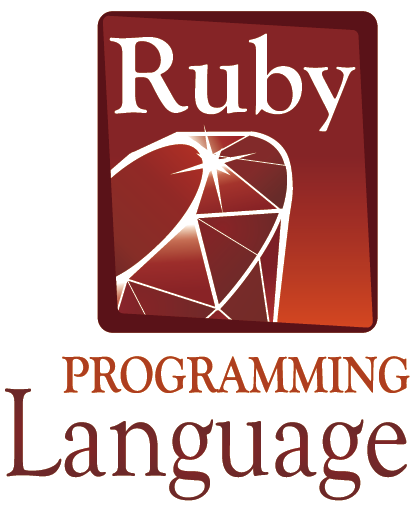
\includegraphics[height=5cm]{gfx/ruby}
\hspace{0.5cm}

\includegraphics[height=5cm]{gfx/ror}
\caption[Ruby and Ruby on Rails]{Ruby programming language (left) \\
and Ruby on Rails framework (right).}
\end{figure}

The system sits on top of \emph{Ruby on Rails}
(or \emph{Rails}, in short) \cite{rails} framework.
Rails is a mature and stable framework that has been in
web development for decades \cite[]{railsd}. So it has a great support
and a large community bebind. A great choice for building a sustainable
system.

Rails is capable of both web service and web interface.
By sharing the same algorithm we could provide a service
for both programs (targeted by web service) and humans
(targeted by web interface).
